\documentclass[a0,portrait]{a0poster}
\usepackage{times,colordvi,amsmath,amssymb,amsthm,epsfig,float,color,multicol}
\usepackage{graphics}
\usepackage{hhline}
\usepackage[large]{subfigure}
\usepackage[latin1]{inputenc}
% Klassen m� alltid v�re a0poster, og den kan ta en rekke opsjoner:
%
% landscape
% portrait
% a0b   ``DIN A0 big''. Brukes til � f� full bredde p� HP Designjet
%                       650C. Dette valget er standard.
% a0    ``DIN A0''.
% a1    ``DIN A1''.
% a2    ``DIN A2''.
% a3    ``DIN A3''.
% draft                 Gj�r om til A4 for testutskrift.
% final                 Gj�r at PS-fila blir i spesifisert st�rrelse;
%                       standard.
% a0poster-klassen st�tter en rekke fontsst�rrelser:
%
% \tiny            12pt
% \scriptsize      14.4pt
% \footnotesize    17.28pt
% \small           20.74pt
% \normalsize      24.88pt
% \large           29.86pt
% \Large           35.83pt
% \LARGE           43pt
% \huge            51.6pt
% \Huge            61.92pt
% \veryHuge        74.3pt
% \VeryHuge        89.16pt
% \VERYHuge        107pt
% N�r du har kj�rt latex 'filnavn.tex', vil det dukke opp en fil til i
% katalogen; 'a0header.ps'. Denne filen m� ligge der n�r du kj�rer
% dvips.
\def \ndte{NDT\&E}
\def \rl{Lamb}
\newcommand{\grad}{\vec{\nabla}}

%%%%%%%%%%%%%
%  Lengder: %
%%%%%%%%%%%%%
% For � f� margene fine.
\addtolength{\textwidth}{0.0cm}
\addtolength{\oddsidemargin}{-0.5cm}
% Avstanden mellom kolonnene i multicolumn-mode
\setlength{\columnsep}{1.2cm}
\setlength{\columnseprule}{0.5pt}
%\setlength{\parindent}{0cm}
%\setlength{\parskip}{2ex}
\setlength{\parindent}{1em}
\setlength{\parskip}{0cm}
%%%%%%%%%%%%%%%%%%%%%%%%%%%%%%%
%  Kommando-definisjoner:     %
%%%%%%%%%%%%%%%%%%%%%%%%%%%%%%%
% Ingen side-nummerering
\pagestyle{empty}
% Setter standard skrifttype til � v�re 'phv'; Sans Serif.
%MC commented out next line
%\renewcommand{\familydefault}{phv}
% Setter standard skriftst�rrelse.
%MC commented out next line
%\renewcommand{\normalsize}{\large}
% Definerer 'NTNU-fargen', m�rkebl�tt, for bruk i bl.a. overskrifter.
\definecolor{NTNUBlue}{rgb}{0.0470,0,0.5294}
\makeatletter
\renewcommand{\section}{\@startsection
        {section}%                          % the name 
        {1}%                                % the level
        {0mm}%                              % the indent
        {-0.6\baselineskip}%                % the beforeskip
        {1mm}%                              % the afterskip
        {\Large\color{NTNUBlue}\bfseries}}% % the style
\renewcommand{\subsection}{\@startsection
        {subsection}%                       % the name 
        {2}%                                % the level
        {0mm}%                              % the indent
        {-0.6\baselineskip}%                % the beforeskip
        {1mm}%                              % the afterskip
        {\large\color{NTNUBlue}\bfseries}}% % the style
\renewcommand{\subsubsection}{\@startsection
        {subsubsection}%                    % the name 
        {3}%                                % the level
        {0mm}%                              % the indent
        {-0.6\baselineskip}%                % the beforeskip
        {1mm}%                              % the afterskip
        {\large\color{NTNUBlue}\bfseries}}% % the style
\makeatother
\newcommand{\T}{{\cal T}} 
\newcommand{\AG}{{\sc AnaGraph }}
\def\bP{\mathbb{P}}
\def\bE{\mathbb{E}}

%%%%%%%%%%%% Her begynner selve dokumentet %%%%%%%%%%%%%%%
\begin{document}
\begin{center}
\parbox{0.98\textwidth}{
\begin{center}
\LARGE
\sf
PASC Co-design Project:  {\em Towards the HPC-inference of causality networks from multiscale economical data}
\end{center}
}
\end{center}
\begin{center}
\parbox{0.48\textwidth}{
    \small
    \begin{center}
    Illia~Horenko, Patrick~Gagliardini \\
    Universit\`a Svizzera Italiana \\
    {\tt illia.horenko@usi.ch, patrick.gagliardini@usi.ch}
    \end{center}
}
\parbox{0.48\textwidth}{
    \small
    \begin{center}
    William~Sawyer\\
    Swiss National Supercomputing Centre (CSCS/ETH Zurich) \\
    {\tt william.sawyer@cscs.ch}
    \end{center}
}
\end{center}
% Konstruksjonen (Logo | Overskrift | Logo) plasseres inne i tre \parbox.
% Selve teksten kommer som flere kolonner (multicols).
\vspace{1cm}
\begin{multicols}{2}


\section{Focus of the project}
\label{causality}

{\large Analysis of large amounts of economical data and data-driven inference of causality relations between different
 components of economical systems  is one of the central problems in modern computational finance and economics. The task of proper mathematical description and adequate causality understanding for the economical data is hampered by the multiscale nature of the underlying processes, resulting from the presence of different temporal and spatial, i.e. regional, sectorial and global, scales. }

\noindent
{\large Important challenges are: (i) an investigation of the mutual causality influences of different economic observables and their spatial (e.g., regional) and temporal (e.g., associated with the business cycle) evolution, (ii) identification of the most important exogenous impact factors that play a role in their dynamics, (iii) proper mathematical and statistical description of the influences coming from the unresolved/latent scales and factors. The solution of these problems can be enhanced by  analysis of  a causality network inferred from the data.  This network is a directed weighted graph with edges representing the causality relations between the  different economical variables, exogenous factors, etc. (situated at the vertices of this causality graph). Analysis of this graph would allow to understand the most important features of the underlying complex economical system.
}

\paragraph{\large Milestone questions about the targeted economical data:}

{\large 
{\color{NTNUBlue}
\begin{enumerate}
  \item {Is there a causality relation between different sectors of the economy with respect to the credit risk migrations?'}
  \item {What is the most effective implementation of the multiscale causality inference framework in the embarassingly-parallel case?}
  \item {Are there any statistically-significant causality impacts from other sectors on the companies inside of the `Banking and Finance' sector?}
  \item {Among all of the considered alternatives and platforms, what is the most scalable implementation for multiscale causality inference?}
\end{enumerate}
}
}


\section{Understanding Causality}
\label{causality}

{\large In its purest deterministic sense, there is a causal relationship between events if one implies that another has occurred.  In reality, such causal relationships can generally only be determined from first principles on a small spatial/temporal scale, with little data involvement.  For larger scales and/or larger data involvement, mathematical or statistical models are required from whence causality can be inferred.}

\begin{figure}[H]
    \begin{center}
         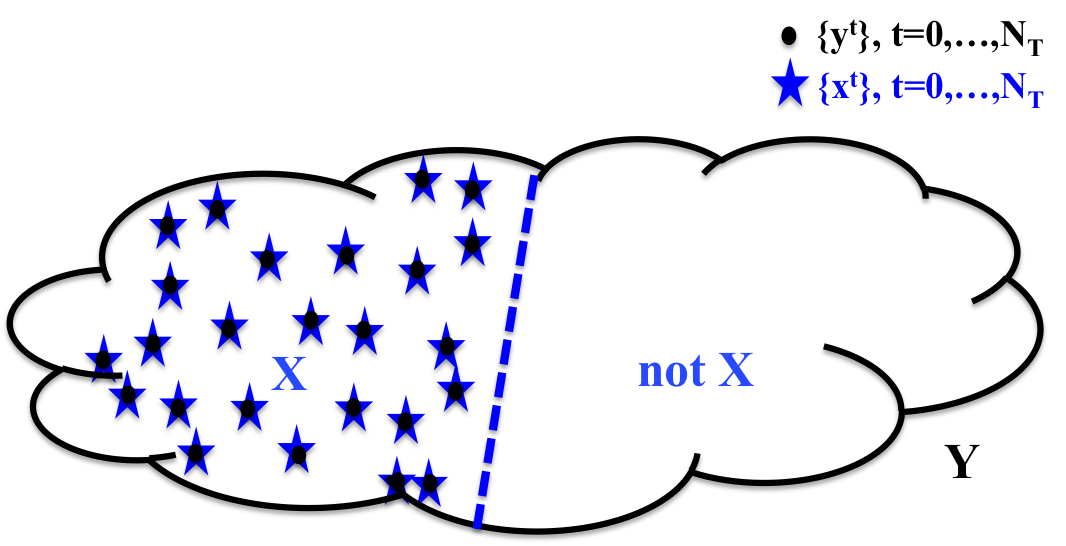
\includegraphics[width=15cm, angle=0, clip = true]{Deterministic_Causality.png}
        \hfil
        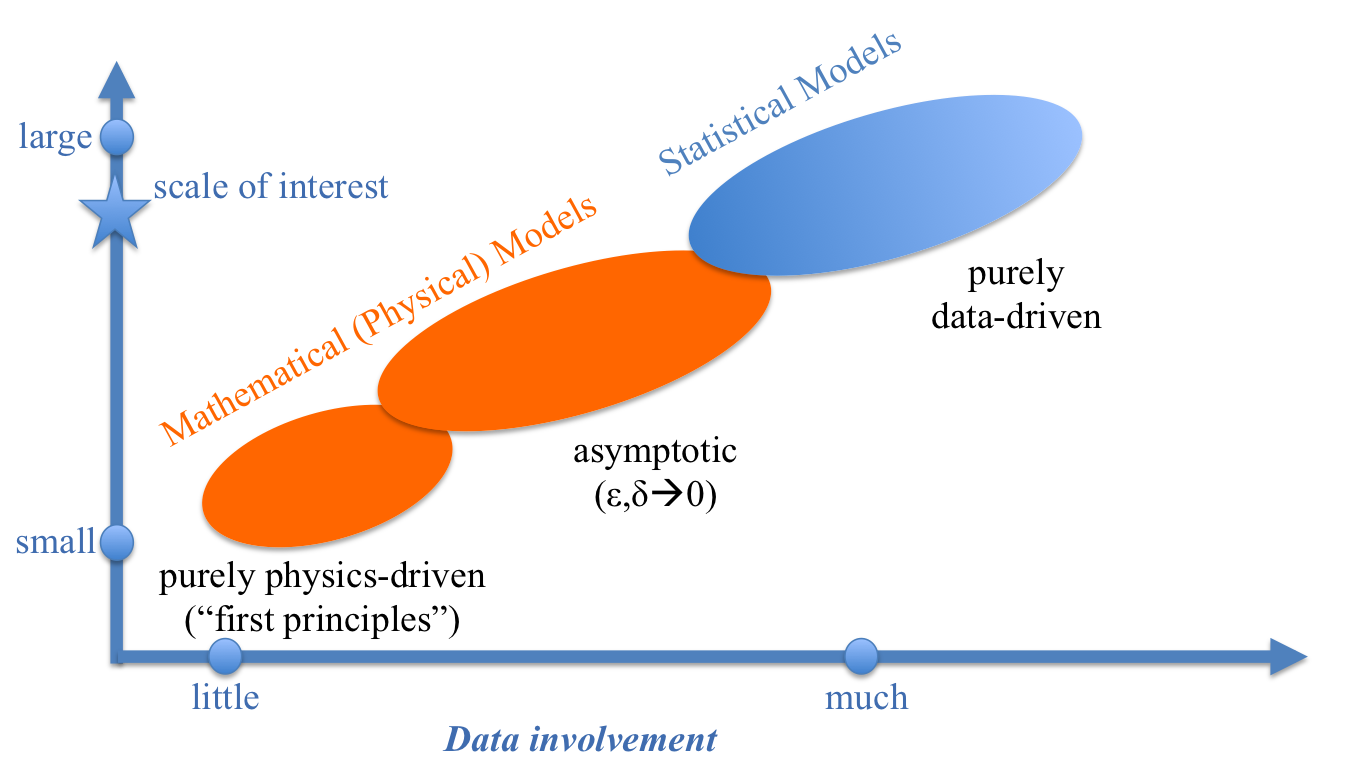
\includegraphics[width=15cm, angle=0, clip = true]{Causality_Model_or_Data_Driven.png}
   \caption{Deterministic Causality (left):  $X$ has a causality impact on $Y$ if for any $t$, event $y^t$ is happening if and only if event $x^t$ happened.  In real applications a data model is required, but the realm of applicability (right) determines whether the causality inference is driven by the model or by the data .}
    \end{center}
\end{figure}

\vspace{-1.0cm}
\paragraph{\large Granger Causality:}  {\large The standard causality inference measures the ability of predicting the future values of a time series (e.g., $y^{t+\tau}$) using past values of another time series (e.g., $x^t,x^{t-\tau},\dots,x^{t-q\tau}$), where $\tau$ is a time step and $q\tau$ is a maximal time lag \cite{granger69}.  The predictive models that have been deployed first to measure such a causality relation between $y$ and $x$ were linear {\bf A}uto{\bf R}egressive models with e{\bf X}ternal impact factors (ARX-models) \cite{brockwell2002}}:
\begin{eqnarray}
\label{eq:ARX}
y^{t+\tau}&=&\mu+\sum_{i=0}^p A_iy^{t-i\tau}+\sum_{j=0}^q B_jx^{t-j\tau}+\sigma\left(t\right),
\end{eqnarray}
{\large where $\{\mu,A_0, A_1,\dots,A_p,B_0, B_1,\dots,B_q\}$ are the ARX-model parameters that can be estimated from the available time series for $x$ and $y$ (e.g., deploying the maximum likelihood method) and $\sigma\left(t\right)$ is some stochastic noise process \cite{brockwell2002}. Then, the variable $x$ has a Granger causality relation to the variable $y$ if and only if at least one of the $B_j$ is statistically-significantly different from zero.}

\paragraph{\large Limitations:} {\large Granger causality may lead to biased results.  This bias might be amplified and lead to a completely wrong inference of the causality relations from the data, if the underlying model assumptions of standard causality inference methods (e.g., like the intrinsic linearity of the Granger causality measures) are not fulfilled.}

\section{Probabilistic (Bayesian) Causality}

{\large In contrast to typical applications from computational sociology (where the underlying network/graph is mostly available explicitly, e.g., in the form of a social network directly describing the observed connections and relations between the individuals), in a context of economical data these causality network structures are often implicit, difficult to measure, and need to be inferred from the very large sets of available data.  The law of total probability can assist us:}

\paragraph{\large Law of Total Probability:} 
  {\large If $B_1, B_2, B_3,\cdots$ is a partition of the sample space $S$, then for any event $A$ we have $P(A)=\sum_{i} P(A \cap B_i)=\sum_{i} P(A | B_i) P(B_i)$. }

\vspace{0.5cm}
\noindent
{\large In this project we investigate the case that both $X$ and $Y$ are driven by an (unobserved) process $U$ with different lags, e.g., unresolved scale impacts. We start by defining the probability vectors $\Lambda(t)=(\bP\left[y^t|x_1^t \text{ and } u^t \right],\dots,\bP\left[y^t|x_n^t \text{ and } u^t\right],$ $ \bP[y^t \text{  and not one of } x_i^t])$,  $P_x^t=\left(\bP\left[x_1^t \text{ and } u^t \right],\dots,\bP\left[x_n^t \text{ and } u^t \right],1\right)$ and a variable $P^t_y=\bP\left[y^t \right] $. Then the probability of observing $y^t$ together with $x_1^t,\dots,x_n^t$ and $u^t$ can be written as a scalar product of these two vectors:}

\begin{equation}
\label{eq:full_prob}
P_y^t = \Lambda^{\dagger}(t)P^t_x,
\end{equation}

\begin{figure}[H]
    \begin{center}
        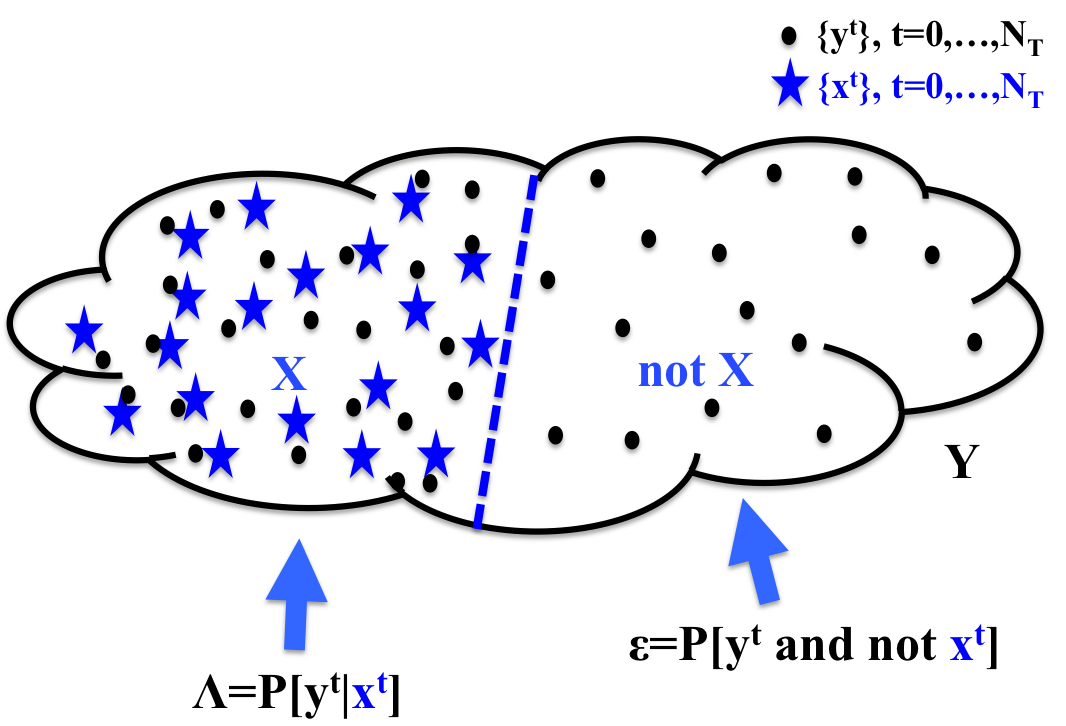
\includegraphics[width=13cm, angle=0, clip = true]{Bayesian_Causality_1.png}
        \hfil
        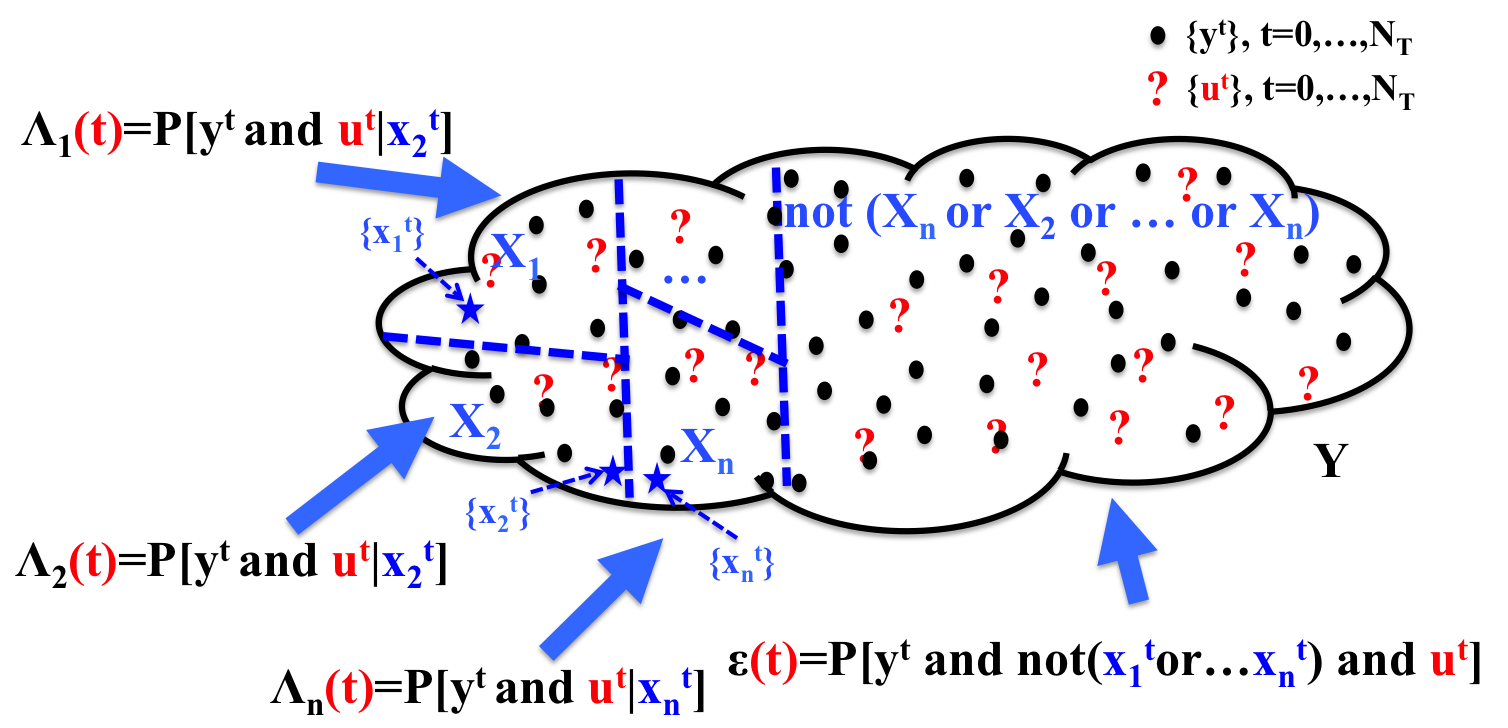
\includegraphics[width=17cm, angle=0, clip = true]{Bayesian_Causality_2.png}
    \caption{The simplest statistical causality model (left) is $P[y^t] = {\bf \Lambda} P[x^t] + \varepsilon$, with $\Lambda \simeq 0$ implying no causality impact of $X$ on $Y$.  The law of total probability  allows a partition (right):  $P[y^t \hat u^t] = \Lambda_1(t) P[x_1^t] + \Lambda_2(t) P[x_2^t]  + \ldots + \Lambda_n(t) P[x_n^t]$, with  $\Lambda_i \simeq 0$ implying no causality impact of  $X_i$ on $Y$.}
    \end{center}
\end{figure}



\section{Algorithm:  approximation through well-posed lower bound}
\label{approx}

{\large Assuming $y^t$ being statistically-independent in $t$  sequence of binary variables or observed probabilities (conditioned on the knowledge of variables $x$ and $u$), inference of both the unknown causality vector $\Lambda(t)$ and of the unknown probability process $P_y^t$ for the discrete state model  (\ref{eq:full_prob}) can be done via a maximisation w.r.t.~$\Lambda(t)$ of the following log-likelihood functional :}

\begin{equation}
\label{eq:loglik}
\mathcal{L}=\max_{\Lambda} \left( \sum_{t=0}^{N_T}\left[\left(1-y^t\right)\ln\left(1-\Lambda^{\dagger}(t)P_x^t\right)
+y^t\ln\left(\Lambda^{\dagger}(t)P^t_x\right)\right] \right).
\end{equation}

\noindent
{\large This problem is unfortunately ill-posed.  The central challenge is to formulate the investigations of $\Lambda_i$ into a well-posed optimisation problem.  We start with the approximation:} 

$$\Lambda (t) = \sum_{i=1}^{K} \gamma_i^t \Lambda_i \;\; \mbox{with} \;\; \sum_{i=1}^K \gamma_i^t = 1, \;\; \gamma_i^t \ge 0.$$

\noindent
 {\large In \cite{horenko_pnas_2014} the following lower bound for $\mathcal{L}$ was proved:}

\begin{equation}
\label{eq:loglik_lb}
%\begin{multlined}
\mathcal{L} \ge l^\epsilon= \max_{\gamma_i^t,\Lambda_i} \left( \sum_{i=1}^{\mathbf{K}}\left[\sum_{t=0}^{N_T}\gamma^t_i g\left(t,\Lambda_i\right)-\epsilon^2\sum_{j=1}^n\lambda_{i}^{(j)}\right] \right).
%\end{multlined}
\end{equation}

\noindent
{\large with $g\left(t,\Lambda_i\right)=\left(1-y^t\right)\ln\left(1-\Lambda^{\dagger}_iP_x^t\right)+y^t\ln\left(\Lambda^{\dagger}_iP^t_x\right)$, and subject to the constraints:}

\begin{eqnarray}
\label{eq:loglik_lb_con00}
&& \sum_{i=1}^{\mathbf{K}}\gamma_i^t=1,  \gamma_i^t\geq 0 \text{ for all $t$ and $i$,}\\
\label{eq:loglik_lb_con0}
&&0<\sum_{j=1}^n\lambda_{i}^{(j)}< 1,\quad  0\leq\lambda_{i}^{(j)}\leq1, \text{ for all $i$ and $j$,}\\
 \label{eq:loglik_lb_con}
 &&\sum_{t_1,t_2=0}^{N_T}|\gamma_i^{t_1}-\gamma_i^{t_2}|\leq\bar{\mathbf{C}}\left(N_T\right) ,\text{ for all $i$.}
\end{eqnarray}

\noindent
{\large The maximisation of $l^\epsilon$ belongs to the well-posed class of FEM-BV-problems.}

\section{High Performance Computing Implementation}
\label{sec:hpc}

{\large Currently the causality inference algorithm is implemented in Matlab using interfaces to existing optimisation libraries (Fig. below).  This sequential approach is not viable for cases of interest ($> 10,000$ companies/sectors). }

\begin{figure}[H]
\begin{center} \centerline{
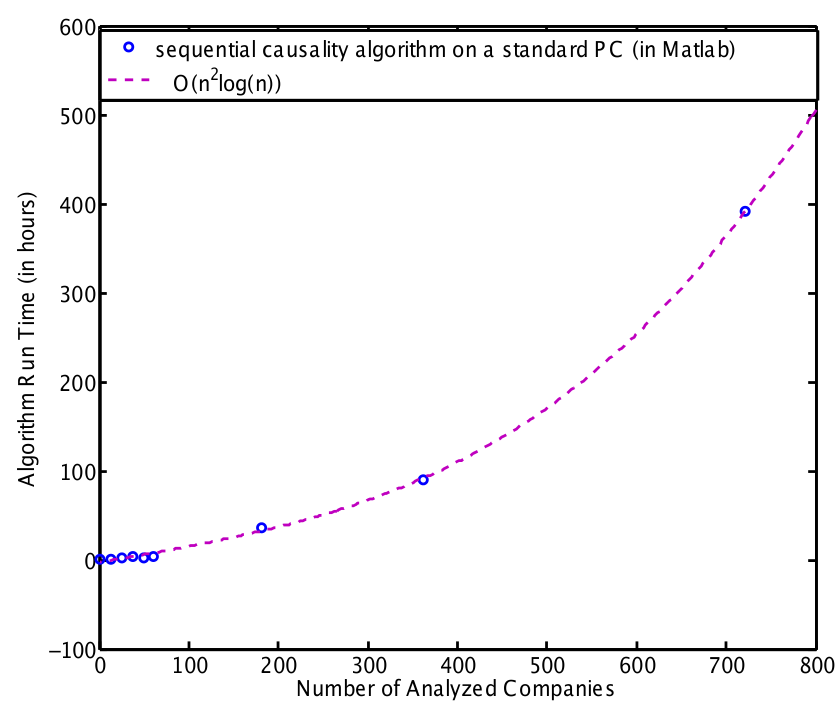
\includegraphics[width=15cm]{run_time_causality_inference.png}
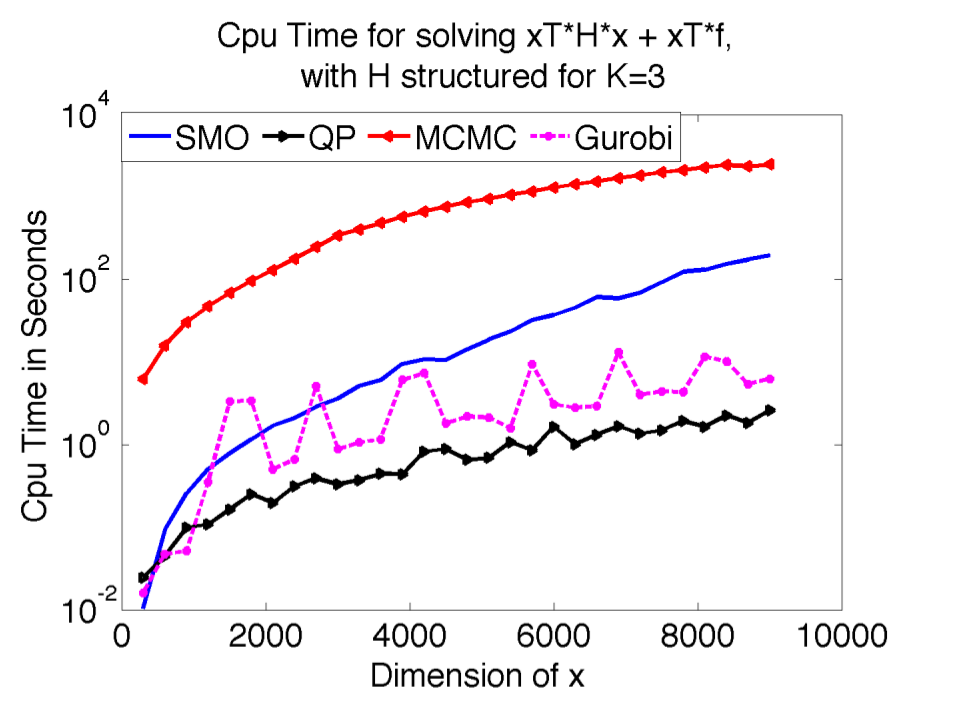
\includegraphics[width=17cm]{Kaiser_structured_smo_mcmc_qp_gurobi_K3.png}
}
 \caption{On left, the run-times of causality inference algorithm in
its current sequential Matlab implementation on an Apple MacBook are shown. The
magenta line is the optimal fit of the $O(n^2 \log n)$-function to this sequence of run times.  On right (courtesy of O. Kaiser), the run times of several variants of the Quadratic Programming (QP) minimisation problem performed in every annealing step of the causality algorithm illustrate a similar time evolution (note log-linear scale), albeit with different leading coefficients. The dimension of x is length of the time series and should not be confused with the $n$. The magenta Gurobi curve yields a slightly better scaling since this library employs OpenMP multithreading, which may scale better for increasing problem size. }
 \end{center} \label{fig:perf}
\end{figure}

\vspace{-0.5cm}
\noindent
{\large Key challenges in the implemention  will be to (i)  exploit distributed memory parallelism inherent in the algorithm, and (ii) to identify and utilise existing numerical libraries which hide the complexity of programming emerging architectures such as GPGPUs and Intel Xeon Phi, instead of trying to program these directly.  Preliminary investigations (Fig. below) reveal potential strong scaling using a hierarchy of libraries.}

\begin{figure}[H]
\begin{center} \centerline{
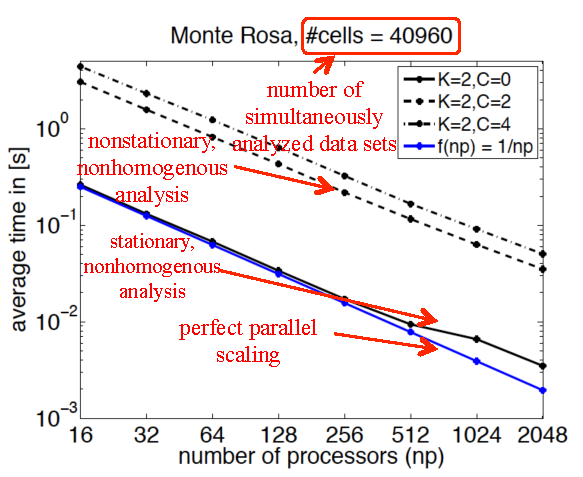
\includegraphics[width=12cm]{Scaling.pdf}
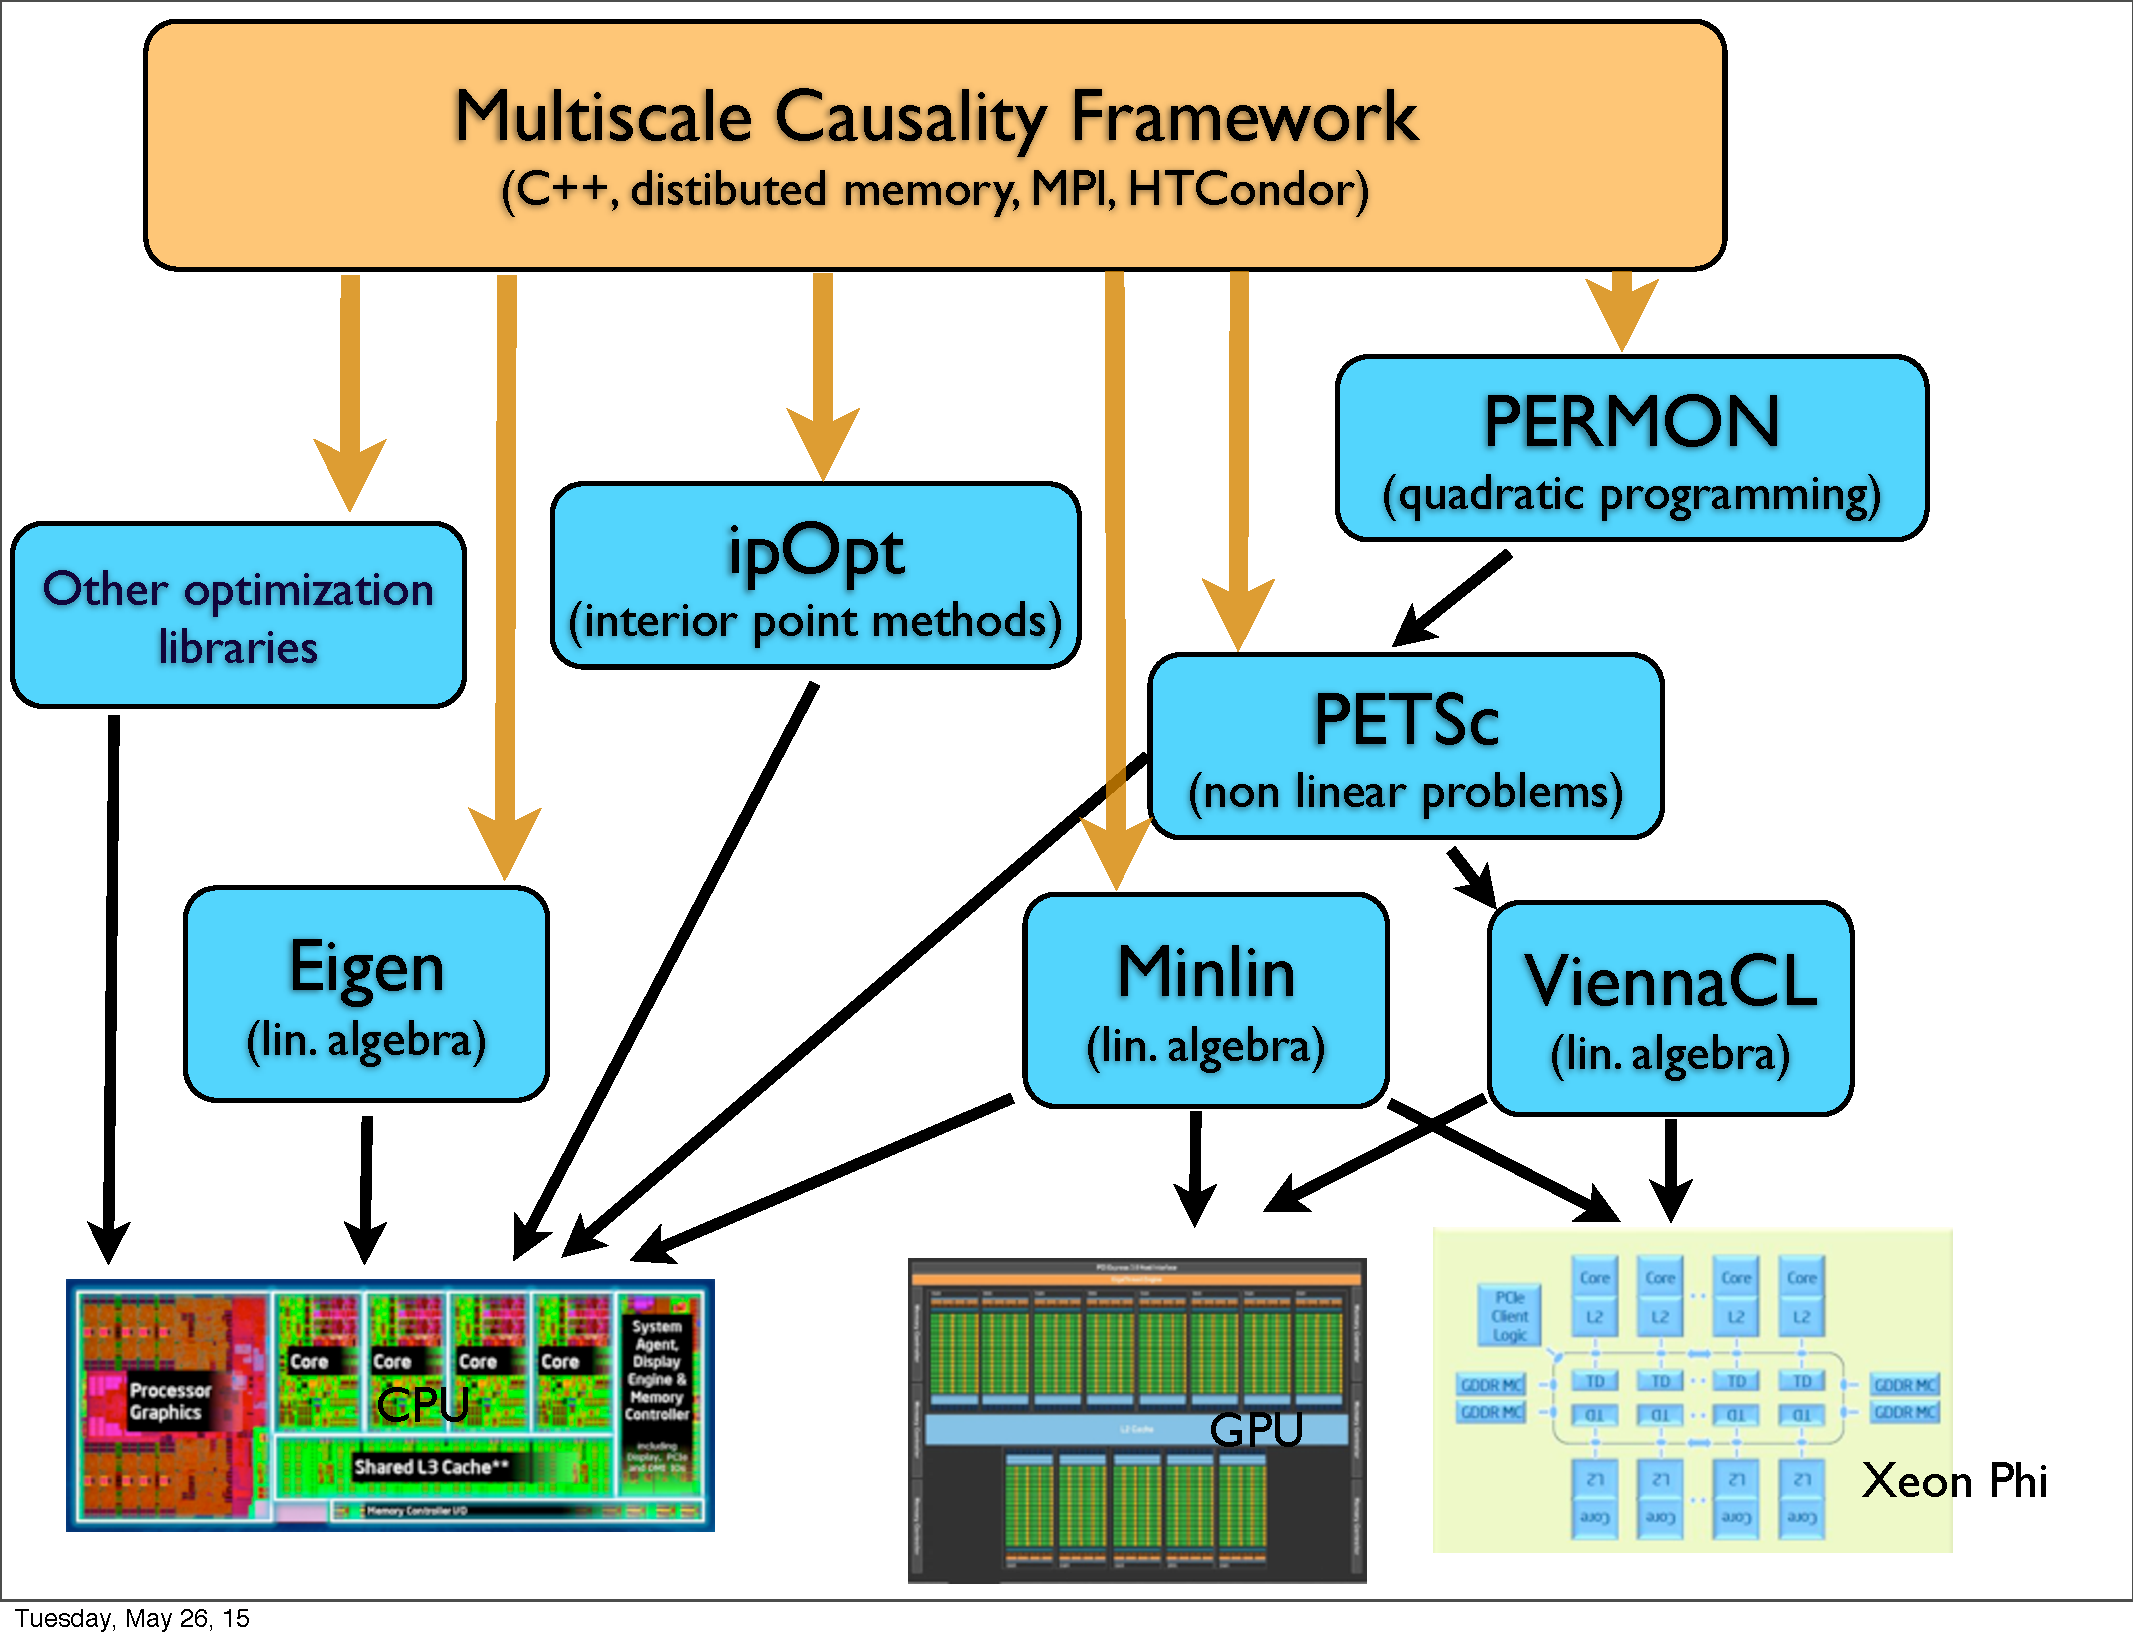
\includegraphics[width=12cm]{Library_Hierarchy.pdf}
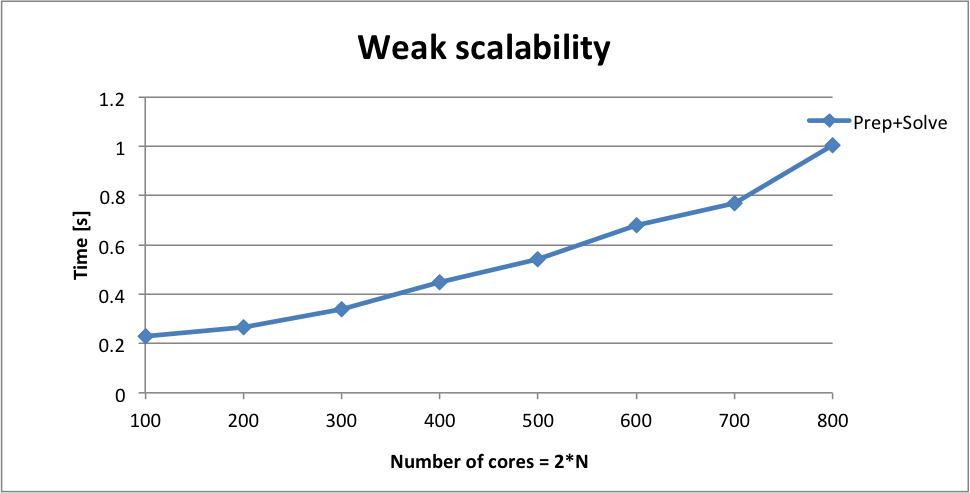
\includegraphics[width=14cm]{FLLOP_weak_scalability.png}}
 \caption{Parallel scaling (left) of the FEM-BV framework in simultaneous (i.e., embarrassingly parallel) analysis of 40960 test data sets (courtesy of P. Metzner). Variable K denotes the number of locally-stationary graphs models that were identified to be in common for all of the data sets, C is the persistency (i.e., a maximal allowed number of switches between these local models pro data set). Note that the computational expense increases for the non-stationary case, but the strong scalability also improves. These preliminary results were obtained on the ``Monte Rosa'' Cray XE6 at CSCS.  A hierarchy of state-of-the-art libraries  (right) contains, e.g., the templated-C++ minimal linear algebra (Minlin) library for dense linear algebra operations on CPUs (OpenMP) and GPUs (cuBLAS), the PERMON (Parallel, Efficient, Robust, Modular, Object-oriented, Numerical) toolbox for constrained optimisation methods, utilising the well-known Portable Extensible Toolkit for Scientific Computation (PETSc) library  for non-linear problems, which in turn utilises the ViennaCL linear algebra backend  to offload linear algebra computation to accelerators. On the far right, the above-mentioned initial results for the above-mentioned QP problem solved with PERMON indicate that weak scaling can still be approached (here on dual 8-core Intel Sandybridge nodes), in spite of the dependencies which make the problem difficult to formulate for parallel platforms. }
 \end{center} \label{fig:Scaling}
\end{figure}

\vspace{-1.0cm}
%
\section{Acknowledgements}
\noindent
\par  The project PI's gratefully acknowledge the financial assistance of the Platform for Advanced Scientific Computing (PASC) for one post doctoral researcher for the period of 2 years {\color{NTNUBlue} (position currently open)}. We would also like to thank Olga Kaiser, Philipp Metzner and the PERMON team for their collaboration in the project.

\par
\bibliography{ams}
\bibliographystyle{apalike}
\begin{thebibliography}{10}
\bibitem{brockwell2002}
P.~Brockwell and R.~Davis.
\newblock {\em Introduction to Time Series and Forecasting}.
\newblock Springer, Berlin, 2002.
\bibitem{granger69}
C.~Granger.
\newblock Investigating causal relations by econometric models and
  cross-spectral methods.
\newblock {\em Econometrica}, 37:424--438, 1969.
\bibitem{horenko_pnas_2014}
S.~Gerber and I.~Horenko.
\newblock On inference of causality for discrete state models in a multiscale
  context.
\newblock {\em Proc. Natl. Acad. Sci. USA (PNAS)}, 2014.

\end{thebibliography}

\end{multicols}
\end{document}





